% Auto-generated by fig_supp_cliques.py — do not edit by hand
\begin{longtable}{ccclp{9.5cm}}
\caption{All cross-species call groups (maximal cliques in the mutual nearest-neighbour graph with $\geq 2$ distinct species). Sorted by number of taxonomic classes, then families, then group size. Icons denote taxonomic class (\protect
\includegraphics[height=0.9em]{../paper_code/icons/cls_amphibia.png}~Amphibia, \protect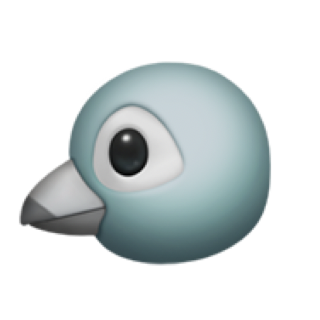
\includegraphics[height=0.9em]{../paper_code/icons/cls_aves.png}~Aves, \protect
\includegraphics[height=0.9em]{../paper_code/icons/cls_mammalia.png}~Mammalia).}\label{tab:supp_cliques}\\
\toprule
Classes & Families & Species & Category & Members \\
\midrule
\endfirsthead
\multicolumn{5}{l}{\textit{(continued from previous page)}} \\
\toprule
Classes & Families & Species & Category & Members \\
\midrule
\endhead
\midrule
\multicolumn{5}{r}{\textit{(continued on next page)}} \\
\endfoot
\bottomrule
\endlastfoot
2 & 2 & 2 & cohesion & 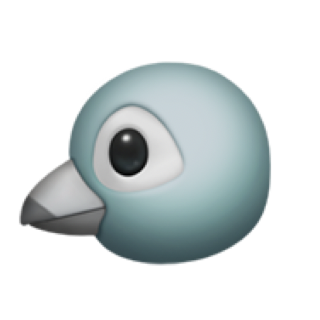
\includegraphics[height=0.9em]{../paper_code/icons/cls_aves.png}~\textit{Taeniopygia guttata} (tet call)\newline 
\includegraphics[height=0.9em]{../paper_code/icons/cls_mammalia.png}~\textit{Loxodonta africana} (rumble) \\
2 & 2 & 2 & danger & 
\includegraphics[height=0.9em]{../paper_code/icons/cls_amphibia.png}~\textit{Allobates femoralis} (advertisement call)\newline 
\includegraphics[height=0.9em]{../paper_code/icons/cls_mammalia.png}~\textit{Elephas maximus} (squeak) \\
2 & 2 & 2 & social & 
\includegraphics[height=0.9em]{../paper_code/icons/cls_amphibia.png}~\textit{Allobates femoralis} (advertisement call)\newline 
\includegraphics[height=0.9em]{../paper_code/icons/cls_mammalia.png}~\textit{Papio anubis} (wa-hoo) \\
2 & 2 & 2 & social & 
\includegraphics[height=0.9em]{../paper_code/icons/cls_amphibia.png}~\textit{Allobates femoralis} (advertisement call)\newline 
\includegraphics[height=0.9em]{../paper_code/icons/cls_mammalia.png}~\textit{Cercopithecus diana} (male general long-distance call) \\
2 & 2 & 2 & social & 
\includegraphics[height=0.9em]{../paper_code/icons/cls_amphibia.png}~\textit{Allobates femoralis} (advertisement call)\newline 
\includegraphics[height=0.9em]{../paper_code/icons/cls_mammalia.png}~\textit{Marmota flaviventris} (whistle) \\
2 & 2 & 2 & cohesion & 
\includegraphics[height=0.9em]{../paper_code/icons/cls_amphibia.png}~\textit{Hyla cinerea} (advertisement call)\newline 
\includegraphics[height=0.9em]{../paper_code/icons/cls_mammalia.png}~\textit{Cercopithecus campbelli} (simple harmonic contact call) \\
2 & 2 & 2 & danger & 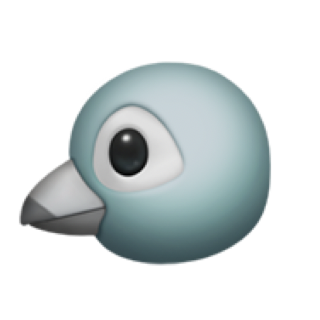
\includegraphics[height=0.9em]{../paper_code/icons/cls_aves.png}~\textit{Poecile carolinensis} (T-slink)\newline 
\includegraphics[height=0.9em]{../paper_code/icons/cls_mammalia.png}~\textit{Papio anubis} (broken grunting) \\
2 & 2 & 2 & distress & 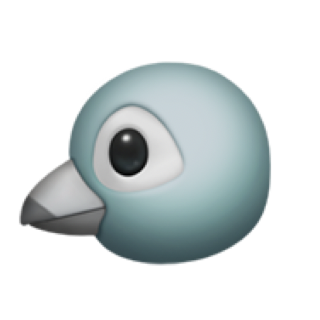
\includegraphics[height=0.9em]{../paper_code/icons/cls_aves.png}~\textit{Poecile carolinensis} (Scream)\newline 
\includegraphics[height=0.9em]{../paper_code/icons/cls_mammalia.png}~\textit{Chlorocebus pygerythrus} (squeal) \\
2 & 2 & 2 & distress & 
\includegraphics[height=0.9em]{../paper_code/icons/cls_amphibia.png}~\textit{Lithobates catesbeianus} (distress call)\newline 
\includegraphics[height=0.9em]{../paper_code/icons/cls_mammalia.png}~\textit{Pan troglodytes} (scream) \\
2 & 2 & 2 & social & 
\includegraphics[height=0.9em]{../paper_code/icons/cls_amphibia.png}~\textit{Engystomops pustulosus} (whine-chuck advertisement call)\newline 
\includegraphics[height=0.9em]{../paper_code/icons/cls_mammalia.png}~\textit{Tursiops truncatus} (burst-pulsed sound) \\
2 & 2 & 2 & social & 
\includegraphics[height=0.9em]{../paper_code/icons/cls_amphibia.png}~\textit{Hyla cinerea} (advertisement call)\newline 
\includegraphics[height=0.9em]{../paper_code/icons/cls_mammalia.png}~\textit{Tursiops truncatus} (burst-pulsed sound) \\
2 & 2 & 2 & foraging & 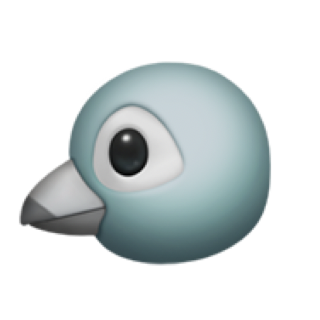
\includegraphics[height=0.9em]{../paper_code/icons/cls_aves.png}~\textit{Taeniopygia guttata} (incubation call)\newline 
\includegraphics[height=0.9em]{../paper_code/icons/cls_mammalia.png}~\textit{Tursiops truncatus} (creak) \\
2 & 2 & 2 & social & 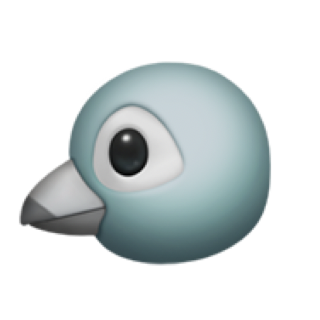
\includegraphics[height=0.9em]{../paper_code/icons/cls_aves.png}~\textit{Taeniopygia guttata} (whine call)\newline 
\includegraphics[height=0.9em]{../paper_code/icons/cls_mammalia.png}~\textit{Rousettus aegyptiacus} (aggression call) \\
2 & 2 & 2 & danger & 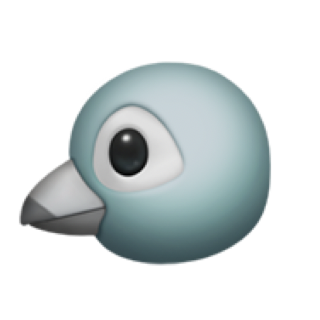
\includegraphics[height=0.9em]{../paper_code/icons/cls_aves.png}~\textit{Gallus gallus} (threat call)\newline 
\includegraphics[height=0.9em]{../paper_code/icons/cls_mammalia.png}~\textit{Canis lupus} (snarl) \\
2 & 2 & 2 & cohesion & 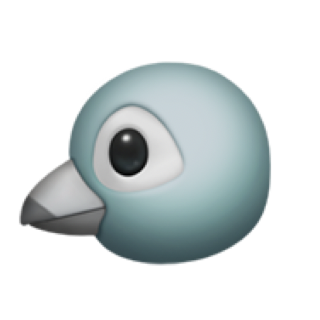
\includegraphics[height=0.9em]{../paper_code/icons/cls_aves.png}~\textit{Gallus gallus} (chick pleasure call)\newline 
\includegraphics[height=0.9em]{../paper_code/icons/cls_mammalia.png}~\textit{Saccopteryx bilineata} (maternal directive call) \\
2 & 2 & 2 & danger & 
\includegraphics[height=0.9em]{../paper_code/icons/cls_amphibia.png}~\textit{Engystomops pustulosus} (whine-chuck advertisement call)\newline 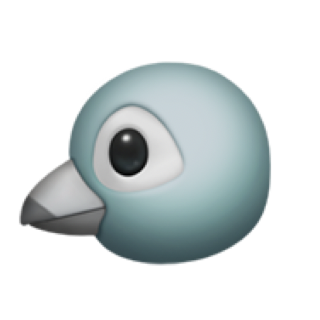
\includegraphics[height=0.9em]{../paper_code/icons/cls_aves.png}~\textit{Parus minor} (jar call) \\
2 & 2 & 2 & danger & 
\includegraphics[height=0.9em]{../paper_code/icons/cls_amphibia.png}~\textit{Hyla cinerea} (advertisement call)\newline 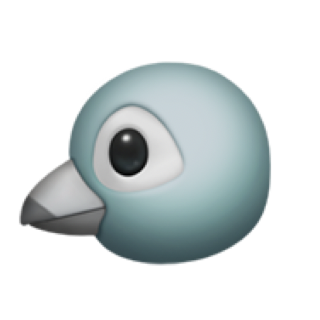
\includegraphics[height=0.9em]{../paper_code/icons/cls_aves.png}~\textit{Parus minor} (jar call) \\
2 & 2 & 2 & danger & 
\includegraphics[height=0.9em]{../paper_code/icons/cls_amphibia.png}~\textit{Lithobates catesbeianus} (distress call)\newline 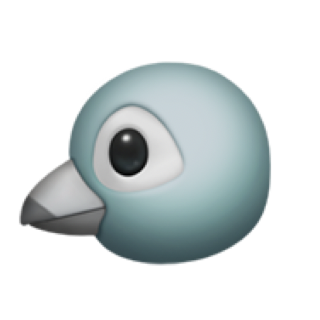
\includegraphics[height=0.9em]{../paper_code/icons/cls_aves.png}~\textit{Parus minor} (jar call) \\
2 & 2 & 2 & danger & 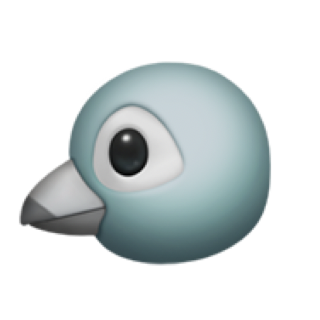
\includegraphics[height=0.9em]{../paper_code/icons/cls_aves.png}~\textit{Parus minor} (jar call)\newline 
\includegraphics[height=0.9em]{../paper_code/icons/cls_mammalia.png}~\textit{Callithrix jacchus} (tsik) \\
2 & 2 & 2 & danger & 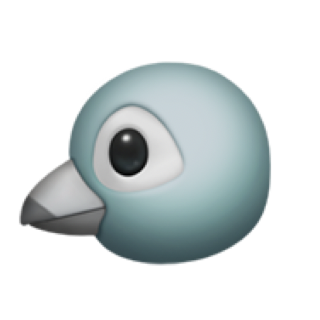
\includegraphics[height=0.9em]{../paper_code/icons/cls_aves.png}~\textit{Parus minor} (ABC call)\newline 
\includegraphics[height=0.9em]{../paper_code/icons/cls_mammalia.png}~\textit{Chlorocebus pygerythrus} (nyow) \\
2 & 2 & 2 & danger & 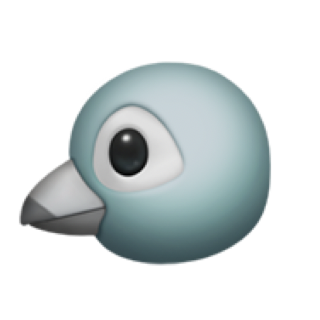
\includegraphics[height=0.9em]{../paper_code/icons/cls_aves.png}~\textit{Parus minor} (ABC call)\newline 
\includegraphics[height=0.9em]{../paper_code/icons/cls_mammalia.png}~\textit{Suricata suricatta} (recruitment call) \\
2 & 2 & 2 & cohesion & 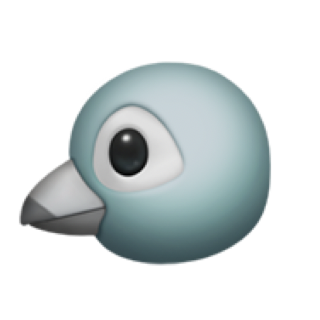
\includegraphics[height=0.9em]{../paper_code/icons/cls_aves.png}~\textit{Taeniopygia guttata} (tet call)\newline 
\includegraphics[height=0.9em]{../paper_code/icons/cls_mammalia.png}~\textit{Suricata suricatta} (close call) \\
2 & 2 & 2 & other & 
\includegraphics[height=0.9em]{../paper_code/icons/cls_amphibia.png}~\textit{Engystomops pustulosus} (whine-chuck advertisement call)\newline 
\includegraphics[height=0.9em]{../paper_code/icons/cls_mammalia.png}~\textit{Suricata suricatta} (sunning call) \\
2 & 2 & 2 & other & 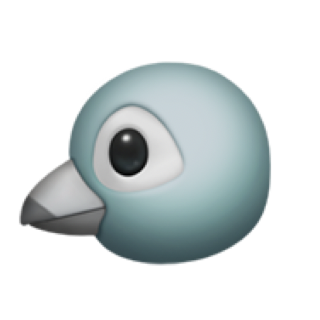
\includegraphics[height=0.9em]{../paper_code/icons/cls_aves.png}~\textit{Taeniopygia guttata} (whine call)\newline 
\includegraphics[height=0.9em]{../paper_code/icons/cls_mammalia.png}~\textit{Suricata suricatta} (sunning call) \\
2 & 2 & 2 & danger & 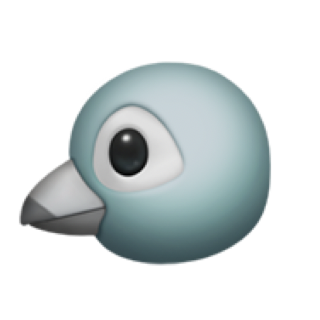
\includegraphics[height=0.9em]{../paper_code/icons/cls_aves.png}~\textit{Gallus gallus} (ground-predator cackling alarm)\newline 
\includegraphics[height=0.9em]{../paper_code/icons/cls_mammalia.png}~\textit{Cercopithecus nictitans} (hack) \\
2 & 2 & 2 & danger & 
\includegraphics[height=0.9em]{../paper_code/icons/cls_amphibia.png}~\textit{Lithobates catesbeianus} (distress call)\newline 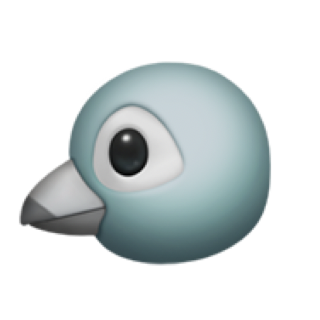
\includegraphics[height=0.9em]{../paper_code/icons/cls_aves.png}~\textit{Gallus gallus} (threat call) \\
1 & 2 & 2 & cohesion & 
\includegraphics[height=0.9em]{../paper_code/icons/cls_mammalia.png}~\textit{Loxodonta africana} (rumble)\newline 
\includegraphics[height=0.9em]{../paper_code/icons/cls_mammalia.png}~\textit{Pan troglodytes} (hoo) \\
1 & 2 & 2 & cohesion & 
\includegraphics[height=0.9em]{../paper_code/icons/cls_mammalia.png}~\textit{Loxodonta africana} (rumble)\newline 
\includegraphics[height=0.9em]{../paper_code/icons/cls_mammalia.png}~\textit{Cercopithecus campbelli} (boom) \\
1 & 2 & 2 & distress & 
\includegraphics[height=0.9em]{../paper_code/icons/cls_mammalia.png}~\textit{Loxodonta africana} (roar)\newline 
\includegraphics[height=0.9em]{../paper_code/icons/cls_mammalia.png}~\textit{Theropithecus gelada} (wobble) \\
1 & 2 & 2 & distress & 
\includegraphics[height=0.9em]{../paper_code/icons/cls_mammalia.png}~\textit{Loxodonta africana} (roar)\newline 
\includegraphics[height=0.9em]{../paper_code/icons/cls_mammalia.png}~\textit{Pan troglodytes} (scream) \\
1 & 2 & 2 & distress & 
\includegraphics[height=0.9em]{../paper_code/icons/cls_mammalia.png}~\textit{Loxodonta africana} (bark)\newline 
\includegraphics[height=0.9em]{../paper_code/icons/cls_mammalia.png}~\textit{Marmota flaviventris} (pup scream) \\
1 & 2 & 2 & other & 
\includegraphics[height=0.9em]{../paper_code/icons/cls_amphibia.png}~\textit{Lithobates catesbeianus} (advertisement call)\newline 
\includegraphics[height=0.9em]{../paper_code/icons/cls_amphibia.png}~\textit{Engystomops pustulosus} (whine-chuck advertisement call) \\
1 & 2 & 2 & cohesion & 
\includegraphics[height=0.9em]{../paper_code/icons/cls_mammalia.png}~\textit{Elephas maximus} (growl)\newline 
\includegraphics[height=0.9em]{../paper_code/icons/cls_mammalia.png}~\textit{Chlorocebus pygerythrus} (grunt) \\
1 & 2 & 2 & cohesion & 
\includegraphics[height=0.9em]{../paper_code/icons/cls_mammalia.png}~\textit{Elephas maximus} (croak-rumble)\newline 
\includegraphics[height=0.9em]{../paper_code/icons/cls_mammalia.png}~\textit{Theropithecus gelada} (wobble) \\
1 & 2 & 2 & distress & 
\includegraphics[height=0.9em]{../paper_code/icons/cls_mammalia.png}~\textit{Pan paniscus} (scream)\newline 
\includegraphics[height=0.9em]{../paper_code/icons/cls_mammalia.png}~\textit{Callithrix jacchus} (tsik) \\
1 & 2 & 2 & cohesion & 
\includegraphics[height=0.9em]{../paper_code/icons/cls_mammalia.png}~\textit{Pan paniscus} (whistle)\newline 
\includegraphics[height=0.9em]{../paper_code/icons/cls_mammalia.png}~\textit{Tursiops truncatus} (signature whistle) \\
1 & 2 & 2 & cohesion & 
\includegraphics[height=0.9em]{../paper_code/icons/cls_mammalia.png}~\textit{Cercopithecus campbelli} (boom)\newline 
\includegraphics[height=0.9em]{../paper_code/icons/cls_mammalia.png}~\textit{Marmota flaviventris} (tooth chatter) \\
1 & 2 & 2 & cohesion & 
\includegraphics[height=0.9em]{../paper_code/icons/cls_mammalia.png}~\textit{Cercopithecus campbelli} (simple harmonic contact call)\newline 
\includegraphics[height=0.9em]{../paper_code/icons/cls_mammalia.png}~\textit{Suricata suricatta} (close call) \\
1 & 2 & 2 & distress & 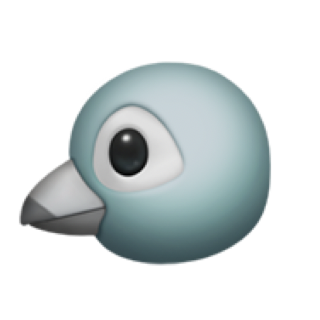
\includegraphics[height=0.9em]{../paper_code/icons/cls_aves.png}~\textit{Poecile carolinensis} (Squeal)\newline 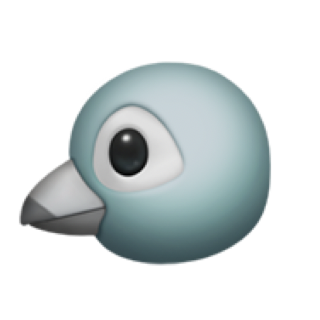
\includegraphics[height=0.9em]{../paper_code/icons/cls_aves.png}~\textit{Corvus corax} (Growl-like) \\
1 & 2 & 2 & distress & 
\includegraphics[height=0.9em]{../paper_code/icons/cls_mammalia.png}~\textit{Pan troglodytes} (scream)\newline 
\includegraphics[height=0.9em]{../paper_code/icons/cls_mammalia.png}~\textit{Theropithecus gelada} (copulation call) \\
1 & 2 & 2 & distress & 
\includegraphics[height=0.9em]{../paper_code/icons/cls_mammalia.png}~\textit{Pan troglodytes} (scream)\newline 
\includegraphics[height=0.9em]{../paper_code/icons/cls_mammalia.png}~\textit{Callithrix jacchus} (tsik) \\
1 & 2 & 2 & cohesion & 
\includegraphics[height=0.9em]{../paper_code/icons/cls_mammalia.png}~\textit{Tursiops truncatus} (signature whistle)\newline 
\includegraphics[height=0.9em]{../paper_code/icons/cls_mammalia.png}~\textit{Crocuta crocuta} (whoop) \\
1 & 2 & 2 & social & 
\includegraphics[height=0.9em]{../paper_code/icons/cls_mammalia.png}~\textit{Tursiops truncatus} (burst-pulsed sound)\newline 
\includegraphics[height=0.9em]{../paper_code/icons/cls_mammalia.png}~\textit{Callithrix jacchus} (tsik) \\
1 & 2 & 2 & foraging & 
\includegraphics[height=0.9em]{../paper_code/icons/cls_mammalia.png}~\textit{Tursiops truncatus} (bang)\newline 
\includegraphics[height=0.9em]{../paper_code/icons/cls_mammalia.png}~\textit{Panthera leo} (woof) \\
1 & 2 & 2 & foraging & 
\includegraphics[height=0.9em]{../paper_code/icons/cls_mammalia.png}~\textit{Tursiops truncatus} (echolocation click train)\newline 
\includegraphics[height=0.9em]{../paper_code/icons/cls_mammalia.png}~\textit{Rousettus aegyptiacus} (echolocation click) \\
1 & 2 & 2 & distress & 
\includegraphics[height=0.9em]{../paper_code/icons/cls_mammalia.png}~\textit{Rousettus aegyptiacus} (isolation call)\newline 
\includegraphics[height=0.9em]{../paper_code/icons/cls_mammalia.png}~\textit{Phyllostomus hastatus} (infant isolation call) \\
1 & 2 & 2 & distress & 
\includegraphics[height=0.9em]{../paper_code/icons/cls_mammalia.png}~\textit{Rousettus aegyptiacus} (isolation call)\newline 
\includegraphics[height=0.9em]{../paper_code/icons/cls_mammalia.png}~\textit{Leptonychotes weddellii} (pup primary call) \\
1 & 2 & 2 & other & 
\includegraphics[height=0.9em]{../paper_code/icons/cls_mammalia.png}~\textit{Rousettus aegyptiacus} (echolocation click)\newline 
\includegraphics[height=0.9em]{../paper_code/icons/cls_mammalia.png}~\textit{Phyllostomus hastatus} (echolocation call) \\
1 & 2 & 2 & cohesion & 
\includegraphics[height=0.9em]{../paper_code/icons/cls_mammalia.png}~\textit{Saccopteryx bilineata} (maternal directive call)\newline 
\includegraphics[height=0.9em]{../paper_code/icons/cls_mammalia.png}~\textit{Phyllostomus hastatus} (infant isolation call) \\
1 & 2 & 2 & cohesion & 
\includegraphics[height=0.9em]{../paper_code/icons/cls_mammalia.png}~\textit{Saccopteryx bilineata} (maternal directive call)\newline 
\includegraphics[height=0.9em]{../paper_code/icons/cls_mammalia.png}~\textit{Leptonychotes weddellii} (pup contact call) \\
1 & 2 & 2 & foraging & 
\includegraphics[height=0.9em]{../paper_code/icons/cls_mammalia.png}~\textit{Saccopteryx bilineata} (echolocation call)\newline 
\includegraphics[height=0.9em]{../paper_code/icons/cls_mammalia.png}~\textit{Phyllostomus hastatus} (echolocation call) \\
1 & 2 & 2 & danger & 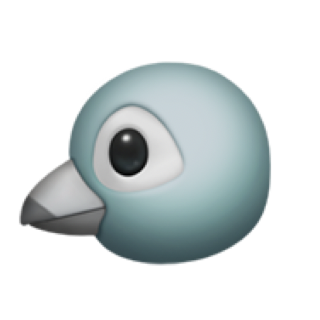
\includegraphics[height=0.9em]{../paper_code/icons/cls_aves.png}~\textit{Parus minor} (jar call)\newline 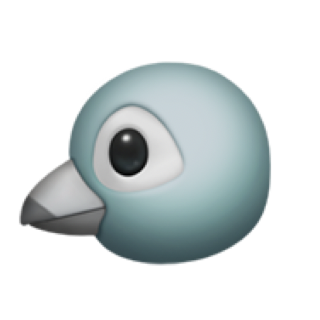
\includegraphics[height=0.9em]{../paper_code/icons/cls_aves.png}~\textit{Gallus gallus} (ground-predator cackling alarm) \\
1 & 2 & 2 & danger & 
\includegraphics[height=0.9em]{../paper_code/icons/cls_mammalia.png}~\textit{Cercopithecus nictitans} (chirp)\newline 
\includegraphics[height=0.9em]{../paper_code/icons/cls_mammalia.png}~\textit{Marmota flaviventris} (whistle) \\
1 & 2 & 2 & cohesion & 
\includegraphics[height=0.9em]{../paper_code/icons/cls_mammalia.png}~\textit{Leptonychotes weddellii} (pup primary call)\newline 
\includegraphics[height=0.9em]{../paper_code/icons/cls_mammalia.png}~\textit{Marmota flaviventris} (pup scream) \\
1 & 1 & 2 & cohesion & 
\includegraphics[height=0.9em]{../paper_code/icons/cls_mammalia.png}~\textit{Loxodonta africana} (rumble)\newline 
\includegraphics[height=0.9em]{../paper_code/icons/cls_mammalia.png}~\textit{Elephas maximus} (rumble) \\
1 & 1 & 2 & foraging & 
\includegraphics[height=0.9em]{../paper_code/icons/cls_mammalia.png}~\textit{Pan paniscus} (grunt)\newline 
\includegraphics[height=0.9em]{../paper_code/icons/cls_mammalia.png}~\textit{Pan troglodytes} (grunt) \\
1 & 1 & 2 & danger & 
\includegraphics[height=0.9em]{../paper_code/icons/cls_mammalia.png}~\textit{Cercopithecus campbelli} (krak)\newline 
\includegraphics[height=0.9em]{../paper_code/icons/cls_mammalia.png}~\textit{Chlorocebus pygerythrus} (chirp) \\
1 & 1 & 2 & danger & 
\includegraphics[height=0.9em]{../paper_code/icons/cls_mammalia.png}~\textit{Papio anubis} (cough-bark)\newline 
\includegraphics[height=0.9em]{../paper_code/icons/cls_mammalia.png}~\textit{Macaca mulatta} (bark) \\
1 & 1 & 2 & danger & 
\includegraphics[height=0.9em]{../paper_code/icons/cls_mammalia.png}~\textit{Macaca mulatta} (bark)\newline 
\includegraphics[height=0.9em]{../paper_code/icons/cls_mammalia.png}~\textit{Chlorocebus pygerythrus} (bark) \\
\end{longtable}
